\documentclass[a4paper]{report}

\usepackage[utf8]{inputenc}
\usepackage[T1]{fontenc}
\usepackage[english, italian]{babel}
\usepackage{amsmath}
\usepackage{hyperref}
\hypersetup{
	colorlinks=true,
	linkcolor=black,
	urlcolor=blue,
	breaklinks=true
}
\usepackage{graphicx}
\graphicspath{ {./images/} }
\usepackage[margin=0.975in]{geometry}
\usepackage[format=hang, font=footnotesize]{caption}
\usepackage{tabularx}
\usepackage{float}

%% document commands
\newcommand{\softwarename}[1]{\underline{#1}}
\newcommand{\softwarecommand}[1]{\textsc{\texttt{\textbf{#1}}}}
\newcommand{\strings}[1]{\textsf{#1}}
\newcommand{\shellcommand}[1]{\\\texttt{\hspace*{0.5cm}#1}\\\\}
\newcommand{\scommand}[1]{\texttt{#1}}	%shell command inline

\title{%
\textbf{Malware Analysis} \\
\large Quasi tutto quello che c'è da sapere}
\author{Luca Gugole}

\begin{document}
\maketitle

\tableofcontents

%%%%%%%%%
%% introduzione
\chapter{Introduzione ai malware e ai tipi di analisi}
La parola \textbf{\textit{malware}} nasce dalla contrazione tra le parole \textit{Malicious} e \textit{Software} e può essere definito come un software o firmware che compie processi non autorizzati che hanno un diverso impatto sulla confidenzialità, integrità o disponibilità di un sistema informativo.
Solo nell'ultimo decennio c'è stato un incremento dell'87\% di infezioni causate da malware. Oggi il 93\% degli attacchi è causato da ransomware.

I malware possono essere utilizzati essenzialmente da tre grandi categorie:
\begin{itemize}
\item Insiders: dipendenti o ex dipendenti che, volendo vendicarsi della propria azienda utilizzano i loro privilegi di amministratore o le loro conoscenze dei sistemi aziendali per compiere attacchi.
\item Cyber criminali: sono criminali che spesso utilizzano i malware per creare un guadagno.
\item Stati-nazione: stati che utilizzano dei malware con lo scopo di arrecare danni ad altri stati e alle loro strutture strategiche, oppure cercando di destabilizzarli.
\end{itemize}

Le modalità per installare i malware all'interno di una macchina di solito si basano quasi esclusivamente sull'ingegneria sociale. ....
%%
\section{Tipologie di malware}
I malware possono essere suddivisi in diverse tipologie:
\subsection*{Virus}
Oggi in disuso, il virus è un malware che ha la capacità di replicarsi sulla macchina su cui viene installato. Per essere eseguita necessità però dell'azione dell'utente che utilizza la macchina. Gli antivirus sono generalmente in grado di identificare i virus.
Si possono distinguere in tre tipologie: le \textit{macro} che arrivano sui computer delle vittime tramite un allegato, i \textit{virus polimorfici} che sono caratterizzati dal fatto che hanno comportamenti diversi in base a quale sistema operativo possiede la vittima, ed i \textit{companion} che si mascherano da programmi legittimi. 
\subsection*{Worm}
Sono simili ai virus ma non hanno bisogno di un'azione dell'utente per essere eseguiti. Inoltre hanno la capacità di diffondesi su vari dispositivi attraverso la rete. Il loro scopo è generalmente quello di installare delle backdoor.
\subsection*{Logic Bomb}
Non molto diffuso, la logic bomb è progettata per compiere dei danni solo quando un determinato evento si verifica. Spesso utilizzato dagli Insider all'interno delle aziende.
\subsection*{Trojans}
Significa "cavallo di Troia" e si presenta come un software sicuro e legittimo quando in realtà viene progettato per compiere azioni malevoli quali operazioni bancarie fraudolente o creare delle backdoor. Ultimamente i trojans vengono utilizzati come vettore per scaricare altri malware sul computer della vittima.
\subsection*{Rootkits}
Sono una tipologia molto pericolosa poichè il loro scopo è dare accesso ai privilegi di amministratore all'attaccante. I rootkit si installano tra il sistema operativo e l'hardware fisico (ad esempio nel kernel), per questo sono difficili da individuare e qualora venissero individuati spesso non possono essere rimossi se non letteralmente distruggendo il disco.
Vengono utilizzati dagli hacker per diversi scopo tra cui quello di assicurarsi di mantenere il loro controllo sulle macchine infette.
\subsection*{Dropper/Downloader}
I dropper e i downloader sono dei malware il cui scopo è quello di portare sulla macchina attaccata altre tipologie di malware scaricandoli dalla rete. I dropper includono il malware stesso all'interno dell'eseguibile come una risorsa, oppure sono contenuti in allegati malevoli.
\subsection*{Key logger}
Molto utilizzata dagli ingegneri sociali, è un malware che ha lo scopo di raccogliere tutti i caratteri digitati sulla tastiera. Tipicamenti i caratteri registrati vengono salvati in un file di testo all'interno del file system e inviati all'attaccante tramite la rete.
\subsection*{Ransomware}
Malware il cui scopo è compromettere la disponibilità dei dati sulla macchina delle vittime. Ciò avviene con la cifratura dei dati personali presenti nelle cartelle e l'unico modo per decifrarli è pagare un riscatto (tipicamente in Bitcoin). Non è mai assicurato il rilascio della chiave di decifratura dopo aver pagato il riscatto, per questo è sempre consigliato di non pagare mai. Il malware più famoso è stato WannaCry.
\subsection*{Bot}
Infettano le macchine per fare in modo di creare una rete di computer infettati dal bot, le cosiddette \textit{botnet}, e spingerle a fare attacchi di Denial of Service (Dos e DDos) e interrompere il servizio di target specifici. Rimangono in attesa del comando dell'attaccante per essere attivati.
Esempi famosi sono Mirai, che colpiva i dispositivi IoT, e Satori.
\subsection*{Cripto Miner}
Tipologia di malware che infetta un dispositivo per installarci sopra un software che mina criptovalute al posto dell'attaccante. Oggi questi malware sembrano essere sempre meno diffusi.

%%
\section{Cyber Kill Chain}
Articola le fasi di un attacco informatico. \`E importante per capire come è avvenuto l'attacco e quali vulnerabilità ha sfruttato. Si compone di 7 fasi.
\begin{enumerate}
\item \textbf{Reconnaissance}: obbiettivo è quello di conosciere il target e raccogliere più informazioni possibili. Ci sono due tecniche principali:
\begin{itemize}
\item Attiva: si raccolgono informazioni interagendo con il target. Alcuni strumenti utilizzati sono, ad esempio, \textit{nmap}, portscanning, vulnerability scanners
\item Passiva: si raccolgono informazioni senza interagire direttamente con il target ma si utilizzano dei servizi esterni. Ad esempio lanciando \textit{whois} o \textit{nslookup}.
\end{itemize}
\item \textbf{Weaponization}: in questa fase si sceglie un modo per attaccare e si crea il mezzo. E\` in questo momento che si crea il malware, chiamato anche "payload". Alcuni strumenti di questa fase sono, ad esempio, Metasploit, Exploit DB o Social Engineering Toolkit.
\item \textbf{Delivery}: in questa fase si adotta un metodo per consegnare il payload malevolo sulla macchina della vittima. Ciò può avvenire ricorrendo alle tecniche di ingegneria sociale, quindi cercando di inviare il malware tramite email, link infetti, chiavette USB e molto altro.
\item \textbf{Exploitation}: fase di esecuzione del malware sulla macchina della vittima. L'esecuzione avviene sfruttando delle vulnerabilità del sistema utilizzato.
\item \textbf{Installation}: in questa fase l'obbiettivo è quello di mantenere il controllo della macchina infetta, raggiungendo così persistenza. Alcune tecniche consistono del sostituire i file DLL di Windows con dei file infetti oppure modificando alcune chiavi di registro.
\item \textbf{Command \& Control (C2)}: questa è la fase in cui l'attaccante comunica con il computer della vittima da remoto stabilendo un canale di comando e controllo.
\item \textbf{Actions on objectives}: fase dell'azione malevola progettata fin dall'inizio. L'attaccante potrebbe cifrare tutti i file del computer oppure raccogliere dati personali della vittima.
\end{enumerate}

\begin{figure}[!ht]
\centering
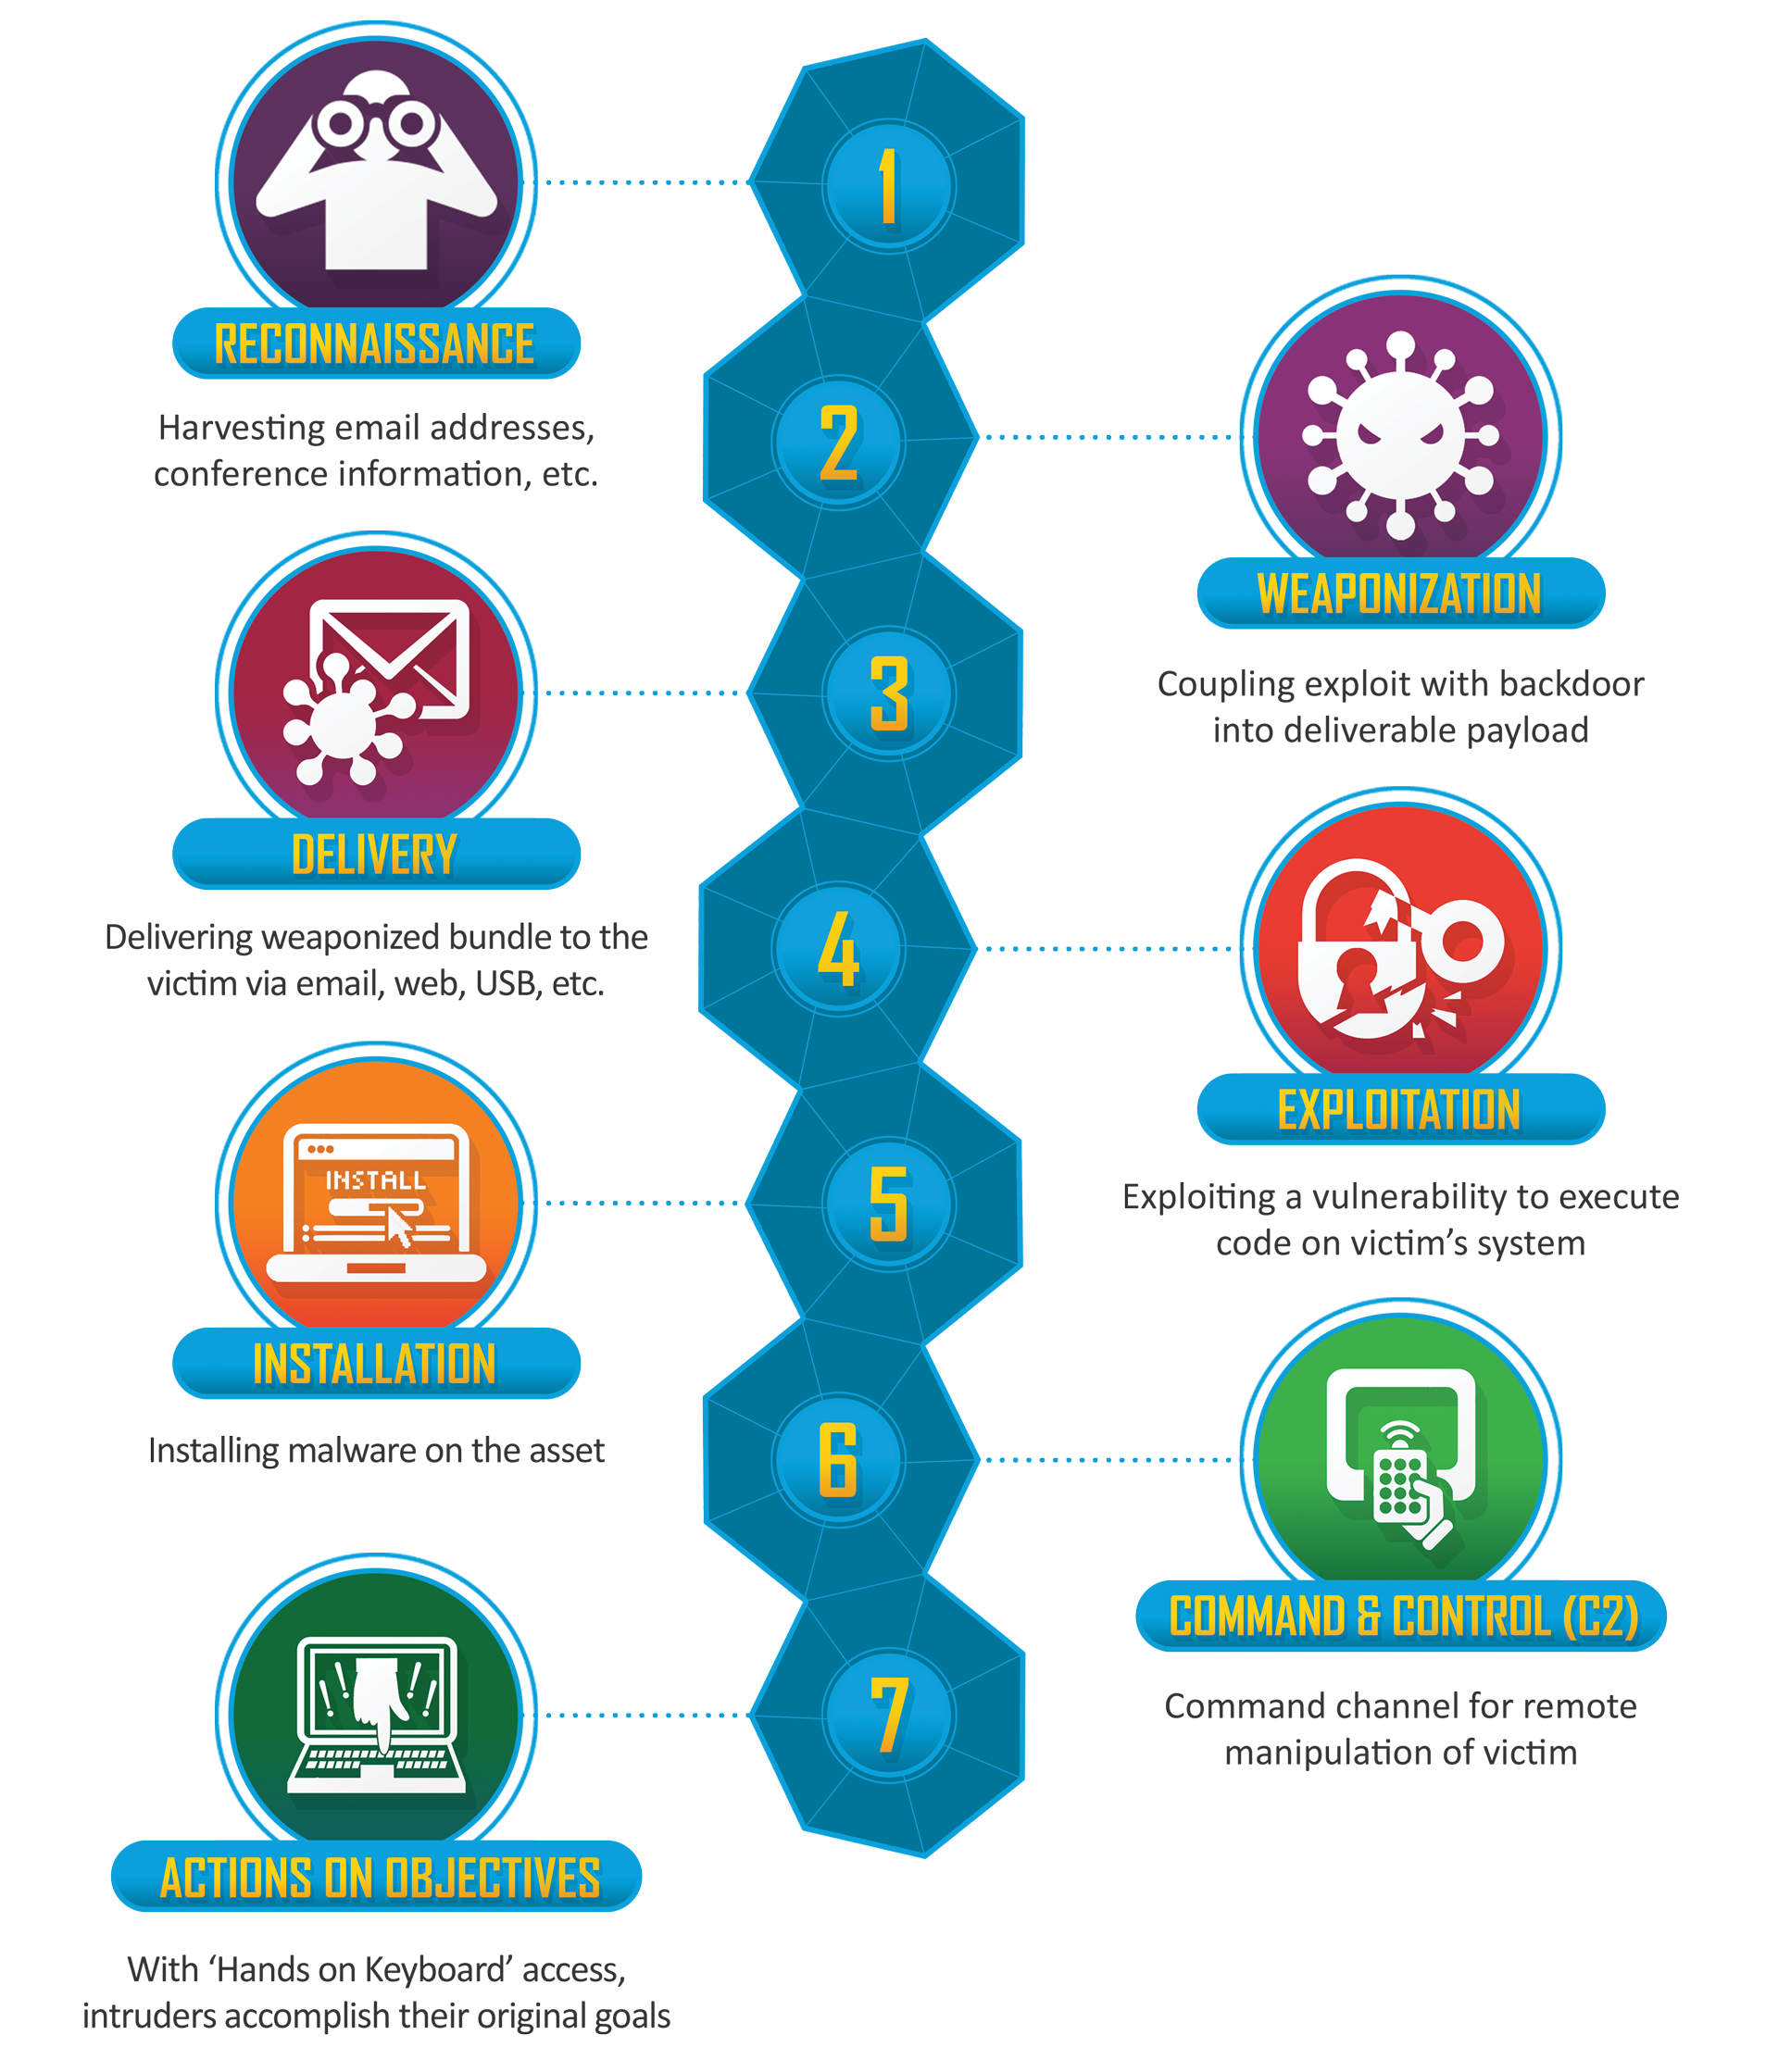
\includegraphics[width=0.7\textwidth]{cyber-kill-chain}
\caption{Schema che mostra i vari passi della Cyber Kill Chain.}
\end{figure}

%%
\section{Analisi dei malware}
L'analisi di un malware è un processo che consiste principalmente in due fasi: l'\textit{analisi statica} e l'\textit{analisi dinamica}. Con l'analisi statica si cerca di analizzare il malware senza eseguirlo, mentre con l'analisi dinamica lo si esegue per vederne il comportamento. Per capire cosa fa un malware spesso si ripete l'analisi più volte, sia statica che dinamica. I due tipi di analisi possono essere a loro volta suddivisi in \textit{analisi di base} e \textit{analisi avanzata}. Nelle analisi di base si va ad analizzare l'eseguibile senza addentrarsi nel codice in cui è stato scritto, mentre nelle analisi avanzate si eseguono operazioni come il reverse engineering o il debugging del codice malevolo. Per riepilogare i tipi di analisi da eseguire e che saranno illustrati nei prossimi capitoli sono:
\begin{enumerate}
\item Analisi statica di base
\item Analisi statica avanzata
\item Analisi dinamica di base
\item Analisi dinamica avanzata
\end{enumerate}

%%
\section{Comportamenti dei malware}
I malware sfruttano molte tecniche per cercare di mascherare il loro lavoro, non solo alla vittima ma anche ai malware analyst. Alcune di queste tecniche sono il cercare di capire se l'eseguibile sta girando su una macchina reale o su una macchina virtuale e per scoprirlo analizzano inanzitutto la quantità di risorse dedicate al sistema in termini di CPU, RAM e quantità di disco, inoltre analizzano i programmi installati sul dispositivo, per esempio, se sono presenti strumenti come Regshot oppure ProcessMonitor sanno che stanno girando sulla macchina di un malware analyst mentre se individuano programmi come Office oppure Adobe Reader sanno che la vittima è un normale utente. Tecniche più raffinate sono l'analizzare le date di creazione, di modifica e di accesso dei file, da cui si evince che, se sono troppo recenti, la macchina potrebbe essere stata appena creata con lo scopo di individuare e analizzare il malware in questione. 

Molti malware prima di connettersi alla rete, controllano se la connessione è disponibile. Il malware analyst può tentare di far credere al malware che la connessione sia disponibile utilizzando strumenti come FakeNet e InetSim.

%%
\section{Preparazione dell'ambiente}
Per eseguire l'analisi di un malware è importante preparare un ambiente in cui poterlo eseguire in modo sicuro, isolato e senza rischi per l'analizzatore.
Esistono i cosiddetti malware lab con macchine dedicate e con una rete completamente isolata, ma questo approccio è utilizzato da aziende e grandi organizzazioni.

Altrimenti, è possibile utilizzare delle macchine virtuali che hanno il vantaggio di isolare sia il sistema operativo sia la rete. Con le macchine virtuali si possono inoltre riportare a istantanee precedenti ed eliminare gli effetti di un malware.
La preparazione dell'ambiente virtuale procede come segue:
\subsection*{Scelta del software di virtualizzazione}
Scegliere il software che può fornirci la creazione di macchine virtuali. I software più famosi sono VMware, Hyper-V e VirtualBox. Il primo è un software commerciale e quindi a pagamento (ha una gestione migliore delle risorse per esperti), mentre gli altri due sono free. VirtualBox è quello che verrà utilizzato da qui in avanti all'interno di questo testo.
\subsection*{Creazione di una nuova macchina virtuale}
Per creare una macchina virtuale, in VirtualBox, basta cliccare su Nuova e impostare le caratteristiche che desideriamo, quali capacità del disco, memoria RAM dedicata, core del processore dedicati e stato della rete. In particolare è consigliato impostare come requisiti minimi le seguenti specifiche:
\begin{itemize}
\item Almeno 1 GB di memoria RAM;
\item Almeno 2 core del processore;
\end{itemize}
Meglio se le specifiche assegnati si avvicinano il più possibile a quelle di una macchina reale, poichè esistono delle categorie di malware che, per rendere più difficile il lavoro del malware analyst, cercano di capire se si trovano su macchine reali o virtuali e cambiare il loro comportamento.
\subsection*{Installazione del sistema operativo}
Prima di procedere all'installazione del sistema operativo sulla macchina, bisogna scaricare l'immagine ISO per l'installazione. Se si tratta di distribuzioni Linux o comunque sistemi open source, le immagini sono scaricabili gratuitamente, mentre per altri sistemi proprietari come Windows (il sistema che si userà in questo testo) è possibile reperire delle versioni per sviluppatore attive per un tempo limitato. \` Microsoft dà la possibilità di scaricare una macchina virtuale completa all'indirizzo: https://developer.microsoft.com/en-us/microsoft-edge/tools/vms.

Si può decidere se installare gli aggiornamenti o meno del sistema operativo; questo per fare in modo di avere una particolare vulnerabilità risolta  nel tempo da un particolare aggiornamento.

Su Windows bisogna disabilitare Windows Defender, sia in real time protection che in cloud protection. Questo perchè anche i tool utilizzati possono essere visti come malevoli.
\subsection*{Installazione dei software per l'analisi dei malware}
L'installazione degli strumenti per l'analisi dei malware può avvenire manualmente, installando i software desiderati. ecc.... su github script python che installa tutti i tool.
\subsection*{Configurazione della rete}
Configurare l'opzione di rete Host-Only (scheda solo host), per impedire al malware di diffondersi attraverso la rete e infettare dispositivi al di fuori della macchina virtuale. Con quest'opzione la rete sarà confinata solamente all'interno della macchina.
\subsection*{Creazione di un istantanea}
Prima di iniziare la prima analisi, è necessario catturare un'istantanea della macchina per poter ripristinare la macchina ad ogni nuova analisi.

%%
\section{Reperire i malware}
Per esercitarsi è possibile scaricare alcuni esempi di malware da diversi siti:
\begin{itemize}
\item Hybrid Analysis
\item ANY.RUN
\item VirusBay
\item VirusShare
\item VirusSign
\item https://zeltser.com/malware-sample-sources/
\end{itemize}

%%%%%%%%%%%%%%
%% analisi statica di base
\chapter{Analisi statica di base}
Nell'analisi statica di base il file malevolo viene analizzato senza essere eseguito. Si differenzia dall'analisi statica avanzata per il fatto che non si vanno a visualizzare le istruzioni del codice malevolo ma si visualizza solo la sua signature. In questo tipo di analisi si vanno, ad esempio, a verificare le stringhe presenti nel file PE. Viene utilizzata per capire la tipologia di file che stiamo analizzando, anche per evitare che alcuni malware si nascondano sotto altre tipologie di file.

Con l'analisi statica di base si va a vedere se un file è effettivamente un malware, se è impacchettato oppure no, quali librerie importa, quali servizi di sistema utilizza e se modifica o no chiavi di registro.

Il tipico processo svolto durante l'analisi statica di base è l'analisi delle stringhe.

%%
\section{Identificazione del file}
Determinare l'effettiva estensione del file è una delle parti principali di questa analisi. Gli hacker tentano infatti di dare una doppia estensione ai file per cercare di mascherare la vera estensione .exe facendo credere che siano ad esempio dei file PDF, documenti di testo o qualsiasi altra cosa appaia innocua.

Alcune volte gli attaccanti mascherano i malware da archivi autoestraenti: con un programma apposito (ad esempio con WinRar) creano un archivio che contiene il malware e scrivono uno script da eseguire all'apertura dell'archivio, in questo modo quando l'utente aprirà il file che sembrerà in tutto e per tutto un archivio compresso, lo script tirerà fuori il malware e lo eseguirà.

L'identificazione di un eseguibile di Windows avviene attraverso l'analisi della signature. In particolare un eseguibile di Windows avrà sempre i primi due bytes dedicati alle lettere \strings{MZ} in codifica ASCII, mentre un PDF inizierà sempre con \strings{\%PDF-}. Un archivio Zip inizia con i bytes dedicati alle lettere \strings{PK}. Questa caratteristica appartiene al DOS Header di ogni file PE, in particolare si tratta del campo e\_magic. Conoscendo questi particolari un programma, come quelli che saranno descritti in questo capitolo, possono facilmente identificare la tipologia di file.

\subsection*{\softwarename{File}}
da scrivere.

\subsection*{\softwarename{ExeInfo PE}}
da scrivere.

\subsection*{\softwarename{PEiD}}
PEiD è uno strumento simile a ExeInfo PE e da informazioni su un file PE analizzato. \\

Per prima cosa, aprire PEiD come amministratore e cliccare sul tasto "..." (tre puntini) per scegliere il file. Una volta scelto il file, la finestra principale di PEiD ci mostra alcune informazioni come... \\

La figura \ref{fig:peid-main} mostra l'analisi di un keylogger.

\begin{figure}[H]
\centering
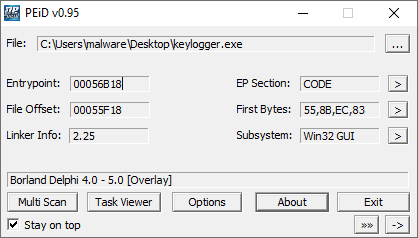
\includegraphics[width=0.65\textwidth]{peid-main}
\caption{Schermata iniziale di PEiD.}
\label{fig:peid-main}
\end{figure}


\subsubsection*{Plugin: Krypto ANALyzer}
Se si dispone del plugin Krypto ANALyzer (o KANAL) è possibile ottenere in una nuova finestra informazioni riguardanti vari algoritmi di codifica e cifratura utilizzati all'interno del malware. Un esempio è mostrato dalla figura \ref{fig:peid-kanal} che ci suggerisce l'utilizzo di ... per il keylogger analizzato sopra.

\begin{figure}[H]
\centering
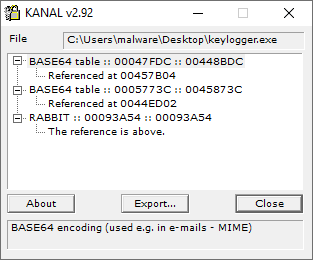
\includegraphics[width=0.50\textwidth]{peid-kanal}
\caption{Plugin KANAL di PEiD.}
\label{fig:peid-kanal}
\end{figure}

\subsection*{\softwarename{TriD}}
da scrivere. Utilizzando i pattern e non le signature non dice esattamente qual è la tipologia di file ma dà una probabilità sulla natura del file.

%%
\section{Calcolo dell'hash}
\`E possibile generare un hash del malware utilizzando diversi algoritmi come MD5, SHA-1, SHA-256, ecc.... Avere l'hash di un file malevolo è utile per farlo analizzare da servizi che cercano di individuarlo nei loro database. Il più famoso è VirusTotal: un servizio online che offre la possibilità di far analizzare un malware dai più conosciuti antivirus in commercio e fornisce i risultati delle analisi e le statistiche. Fornendo a VirusTotal l'hash del codice malevolo è in grado di dire se lo stesso file è già stato individuato in passato come sospetto. VirusTotal è disponibile all'indirizzo: https://virustotal.com.

...immagine virustotal

Alcuni strumenti utili per il calcolo dell'hash di un generico file sono descritti di seguito.

\subsection*{\softwarename{HashMyFiles}}
 
\subsection*{\softwarename{HashCalc}}

\subsection*{\softwarename{ComputeHash}}

%%
\section{Librerie e funzioni importate}
Durante l'analisi statica di base, è importante prestare molta attenzione alle llibrerie Windows, o DLL, importate dal malware. Le librerie più comunemente importate in un eseguibile Windows sono riassunte nella tabella sottostante:
\begin{table}[h!]
\centering
\begin{tabularx}{0.98\textwidth}{
	|  X 
	|  X
	|  X 
	| }
\hline
\textbf{Nome della libreria} & \textbf{Utilizzo da parte del sistema operativo} & \textbf{Utilizzo da parte dei malware} \\ [0.5ex]
\hline\hline
Kernel32.dll & utilizzata da tutti i programmi Windows & Permette al malware di interagire con il file system e la memoria RAM. \\
\hline
Advapi32.dll & manipolare i registri & Utilizzata dai malware per raggiungere persistenza.\\
\hline
User32.dll & gestire l'interfaccia utente & \\
\hline
Gdi32.dll & & \\
\hline
Ntdll.dll & & \\
\hline
WSock32.dll e Ws2\_32.dll & crea connessioni di rete & \\
\hline
Wininet.dll & implementare protocolli di rete HTTP/Https & \\
\hline
\end{tabularx}
\end{table}

Le funzioni più comunemente utilizzate dai malware dipendono dalle operazioni da eseguire.
\subsection*{Operazioni sulla memoria}
\subsubsection*{VirtualAlloc}
\subsubsection*{VirtualProtect}
\subsubsection*{VirtualFree}
\subsection*{Operazioni sui file}
\subsubsection*{CreateFile}
\subsubsection*{ReadFile}
\subsubsection*{WriteFile}
\subsubsection*{DeleteFile}
\subsection*{Operazioni sui registri}
\subsubsection*{RegCreateKey}
\subsubsection*{RegDeleteKey}
\subsubsection*{RegGetValue}
\subsubsection*{RegSetValueEx}
\subsubsection*{RegSetKeyValue}
\subsection*{Operazioni di rete}
connect, accept, send, recv, listen (utilizzata nei malware vettori), gethostbyaddr, gethostbyname,
InternetConnect
InternetReadFile
InternetWriteFile
\subsection*{Altre operazioni}
LoadLibrary
GetProcAddress
IsDebuggerPresent
WriteProcessMemory
CreateRemoteThread

altre: shellExecuteA significa che il malware lancia comandi
itoa: converte indirizzi ip in stringa (??)

%%
\section{Analisi delle stringhe} 
L'analisi delle stringhe consiste nel trovare le possibili stringhe presenti nell'eseguibile compilato e cercare di dare loro dei significati per comprendere se ci troviamo davanti ad un malware e quali sono le sue funzionalità.

Le stringhe che si vanno a cercare sono generalmente di due tipologie in base alla codifica: stringhe \textit{ASCII} o stringhe \textit{Unicode}. Nel caso delle stringhe ASCII ogni carattere della stringa viene codificato con un byte mentre nel caso dell'Unicode ogni carattere ha riservato 2 byte. In entrambe le codifiche ogni stringa viene terminata con il carattere nullo, rappresentato dallo 0.

esempio figura codifica

Gli hacker possono cercare di rendere difficile l'analisi delle stringhe tentando di impacchettare l'eseguibile. L'impacchettamento sarà descritto più avanti.

\subsection*{Stringhe di rete}
All'interno del malware possono trovarsi stringhe che in un certo qual modo indicano un'attività di rete da parte del malware. Queste stringhe possono essere indirizzi IP, nomi di host o indirizzi URL. Qui di seguiti sono indicati alcuni esempi di stringhe di rete:

...

\subsection*{Nomi di file}
Si possono trovare stringhe di nomi di file che possono riguardare file creati dal malware stesso oppure file che il malware va a ricercare all'interno del file system. Molto spesso si trovano stringhe con il nome stesso del malware e ciò indica che il malware tenta di creare copie di se stesso.

\subsection*{Stringhe di librerie}
Si può riconoscere una chiamata a librerie se sono presenti stringhe come: WriteFile, SetRegValue, ecc....

\subsection*{Stringhe di codifica}
La presenza di stringhe del tipo: "inserire stringa" indica l'utilizzo di codifica in Base64. La codifica in base64 infatti utilizza solo un determinato insieme di caratteri che comprende i numeri da 0 a 9, i caratteri da A a Z sia maiuscoli che minuscoli, il simbolo + e /. Una particolarità di questa codifica è che trasforma ogni tre byte in quattro e se la lunghezza finale non è divisibile per quattro si aggiungono i simboli di uguale =.

Per capire quindi se la codifica in base64 è stata utilizzata, dovremmo trovare la stringa A---z0---9+/ oppure stringhe che finiscono con uno o più simboli di uguale.

\subsubsection*{XORSearch}


\subsection*{Chiavi di registro}
Chiavi di registro come stringhe indicano che il malware accede, modifica, crea o cancella chiavi di registro. Ciò viene fatto di solito quando l'eseguibile malevolo vuole raggiungere una certa persistenza sulla macchina.

\subsection*{Altre stringhe}
Altre stringhe che si possono trovare sono stringhe che indicano funzionalità del malware come:

...

\subsection*{Strings}

%%
\section{Data di compilazione}
Coloro che scrivono malware tendono spesso a nascondere la vera data di compilazione che può risultare molto indietro nel tempo oppure addirittura nel futuro. \`E molto utile associare la data di compilazione con altre date all'interno dell'eseguibile come i timestamp associati alle risorse: una grossa differenza in termini di anni può indicare una manomissione della data di compilazione e far crescere il sospetto che il file analizzato sia un file malevolo.

%%
\section{Strumenti per l'analisi statica di base}
L'intera analisi statica di base si basa essenzialmente sull'analisi dei cosiddetti file PE di Windows. Il PE file (si veda l'Appendice A per saperne di più sui PE file) ci può dare molte informazioni sulle librerie importate, lo spazio di memoria allocato per l'eseguibile e molto altro. 

Prima di analizzare come è composto un PE file è importante capire che l'importazione delle librerie utilizzate da un eseguibile può avvenire in tre modi:
\begin{itemize}
\item Statica: tipica dei sistemi Unix, quando si compila un file, le librerie richiamate dal file stesso vengono incluse nell'eseguibile e non è quindi necessario risolvere nessun riferimento.
\item Dinamica: le librerie utilizzate dal file vengono caricate in memoria nel momento in cui l'eseguibile viene caricato in memoria. I nomi e i riferimenti delle librerie da caricare vengono forniti dal campo Import Address Table.
\item Runtime: viene utilizzata principalmente da chi scrive malware. Le librerie vengono caricate nello spazio di memoria allocato dall'esecuzione del malware nel momento in cui vengono chiamate dal malware stesso. Le librerie \textbf{LoadLibrary} e \textbf{GetProcAddress} vengono spesso utilizzate per caricare altre librerie, ed è un forte indicatore del fatto che il malware è stato impacchettato.
\end{itemize}

Ogni file PE è composto da diversi header tra cui DOS Header, PE Header, File Header e Optional Header che sono essenzialmente delle strutture con all'interno diversi campi utili a identificare meglio l'eseguibile analizzato. In particolare, all'interno dell'Optional Header, il campo Magic ci dice se il file è un eseguibile per architetture a 32 bit o a 64 bit, il campo AddressOfEntryPoint indica il puntatore da cui iniziare ad eseguire il codice. I malware possono però effettuare altri controlli prima di questo puntatore quindi non sempre è realmente indicativo dell'inizio delle istruzioni eseguibili. Un altro campo DataDirectory, che contiene il riferimento a diverse tabelle tra cui:
\begin{itemize}
\item Tabella Export Directory: importante se il file eseguibile è una libreria, cioè un DLL. Le funzioni in questa tabella vengono rese disponibile esternamente a chi esegue la libreria.
\item Tabella Import Directory: specifica tutte le librerie importate dal malware. Le librerie da importare sono specificate nel Import Address Table e l'importazione avviene con riferimento dinamico.
\item Tabella Resource Directory: contiene le risorse utilizzate dal file, come le icone.
\item Import Address Table: specifica tutte le librerie che il malware deve importare in memoria. Si tratta di una lista di funzioni per ogni file DLL specificato. Ci possono essere due modi per caricare le librerie contenute nella tabella: il primo consiste da parte del loader nel sostituire il nome contenuto nella tabella con l'effettivo indirizzo della libreria per indicare al malware dove recuperarle; il secondo metodo consiste nel utililzzare un valore ordinale delle funzioni all'interno di una DLL al posto del nome delle funzioni. figura...
\end{itemize}

Un indicatore che ci suggerisce che ci troviamo di fronte ad un malware impacchettato è la presenza di sezioni con nomi diversi da quelli tipici di un PE file e con permessi sia di esecuzione che di scrittura.

Per analizzare un file PE, e completare tutte i tipi di analisi descritti in questo capitolo, si possono utilizzare gli strumenti descritti qui di seguito.

I malware utilizzano le risorse per immagazzinare codice malevolo o file di configurazione. I trojan, che si mascherano da programmi legittimi, nascondono ad esempio dei file PDF malevoli all'interno delle risorse che verranno eseguiti una volta lanciato il trojan.

\subsection*{\softwarename{PEStudio}}
\`E un software pensato appositamente per fare malware analysis, infatti PEStudio tenta già di dare delle indicazioni sui campi analizzati per dire se sono malevoli o no. \`E possibile scaricare una versione PEStudio dal sito "https://www.winitor.com/features" dove sono disponibili sia una versione gratuita che a pagamento.\\

Innanzitutto avviare PEStudio come amministratore, dopodichè importare in PEStudio il file che si vuole analizzare trascinandolo sulla finestra del programma oppure cliccando su \softwarecommand{file > open file} e selezionando dalle cartelle il file da analizzare.\\

Possiamo guardare il contenuto del file header cliccando sulla sezione a sinistra \softwarecommand{file header}. Guardando l'esempio in figura \ref{fig:pestudio-fileheader} notiamo informazioni come la data di compilazione in cui una data di compilazione molto vecchia (in questo caso 2014) potrebbe essere un tentativo di depistaggio da parte dell'attaccante per nascondere il malware. Altre informazioni utili sono \softwarecommand{machine} che indica l'architettura del file (in questo caso x86), il numero di sezioni viene dato da \softwarecommand{section}. Tutte le restanti informazioni riguardano il campo delle caratteristiche.\\

\begin{figure}[H]
\centering
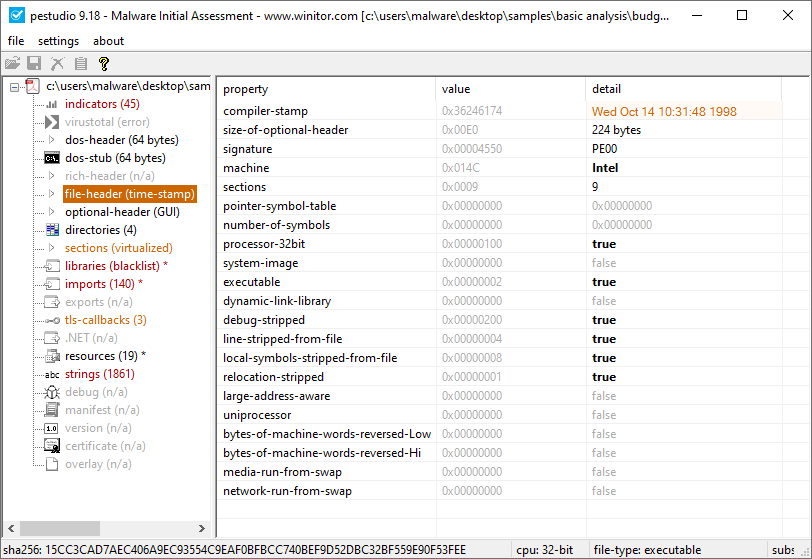
\includegraphics[width=0.65\textwidth]{pestudio-fileheader}
\caption{Schermata che mostra le informazioni estrapolate dal File Header del file caricato in PEStudio.}
\label{fig:pestudio-fileheader}
\end{figure}

Cliccando invece su \softwarecommand{optional header} si possono vedere le informazioni riguardanti l'Optional Header del file PE. La figura \ref{fig:pestudio-optionalheader} mostra il campo magic che contiene PE, l'entry point che ci indica il punto della memoria dove iniziare ad eseguire il codice (in questo caso section:.text indica che il codice parte dalla sezione .text), la dimensione del codice è indicata dal campo size-of-code e l'image base, indicato da image-base indica il punto di caricamento del PE file per il Loader.\\

\begin{figure}[H]
\centering
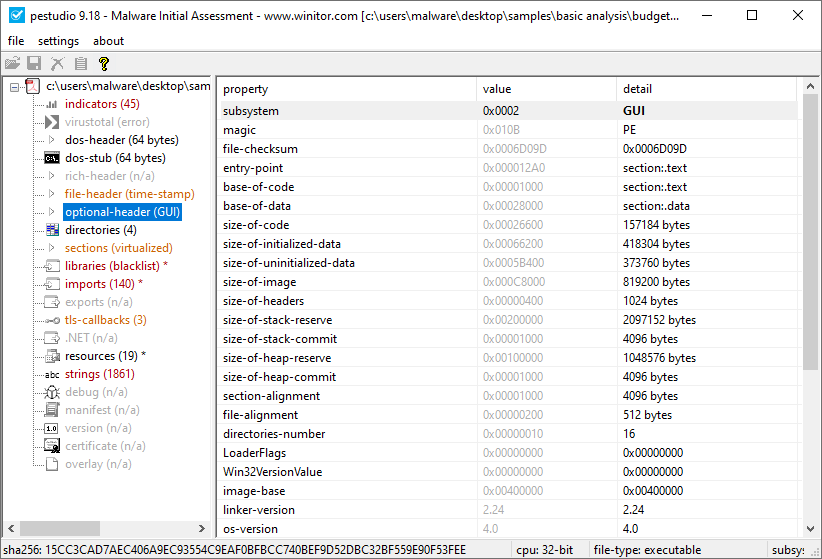
\includegraphics[width=0.65\textwidth]{pestudio-optionalheader}
\caption{Schermata che mostra le informazioni contenute nell'Optional Header del file PE caricato in PEStudio.}
\label{fig:pestudio-optionalheader}
\end{figure}

Una funzionalità importante è la visualizzazione delle sezioni che è possibile cliccando su \softwarecommand{sections} alla sinistra del programma come mostrato dalla figura \ref{fig:pestudio-sections}. Qui è importante guardare se sono presenti sezioni con nomi inusuali e che hanno permessi sia di esecuzione che di scrittura. Il campo name ci indica il nome della sezione e i campi executable, readable e writeable i vari permessi.\\

\begin{figure}[H]
\centering
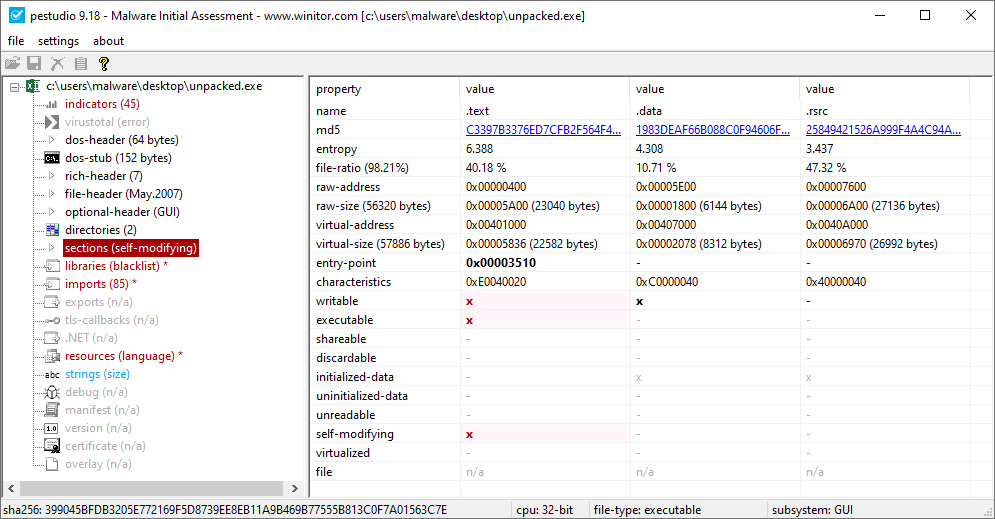
\includegraphics[width=0.65\textwidth]{pestudio-upxunpacked-sections}
\caption{Informazioni riguardanti le sezioni di un file PE in PEStudio.}
\label{fig:pestudio-sections}
\end{figure}

La sezione \softwarecommand{libraries} ci mostra le librerie importate dal PE file malevolo. Nel malware analizzato in figura \ref{fig:pestudio-libraries} notiamo che il file PE importa librerie come \strings{wininet.dll} e \strings{ws2\_32.dll} che indicano un'attività di rete da parte del malware e sono state riconosciute da PEStudio come sospette e quindi segnate da una X in rosso. \\

\begin{figure}[H]
\centering
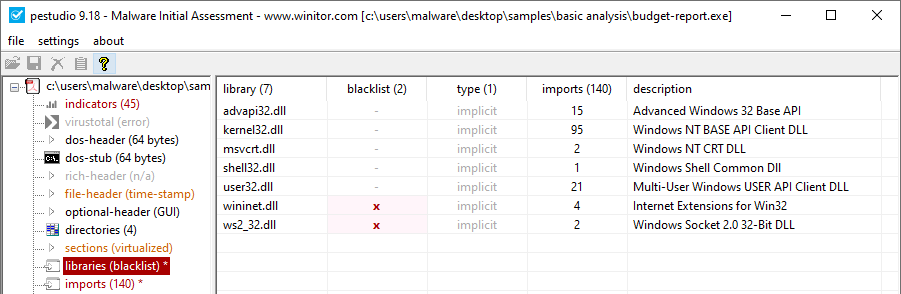
\includegraphics[width=0.65\textwidth]{pestudio-libraries}
\caption{Analisi delle librerie contenute in un file PE attraverso PEStudio}
\label{fig:pestudio-libraries}
\end{figure}

La sezione \softwarecommand{imports} mostra tutte le funzioni importate dal PE file. Anche in questo caso PEStudio ci segna quelle potenzialmente sospette. Dalla figura \ref{fig:pestudio-imports} possiamo notare comunque la presenza di librerie che possono indicare un'azione malevola da parte dell'eseguibile, in particolare: 
... elenco librerie\\

\begin{figure}[H]
\centering
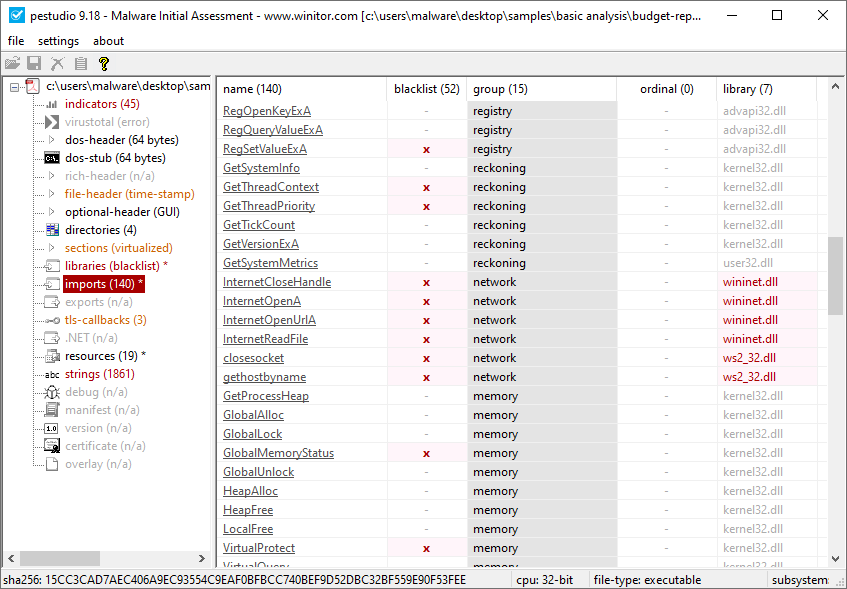
\includegraphics[width=0.65\textwidth]{pestudio-imports}
\caption{Analisi delle librerie importate all'interno di un file PE attraverso PEStudio.}
\label{fig:pestudio-imports}
\end{figure}

Nel campo risorse PE Studio ci fornisce la tipologia del contenuto della risorsa, la signature, la lingua che di solito viene specificata dal programmatore del malware oppure viene impostata in automatico dal compilatore del malware. Nelle risorse di un file PE, un attaccante può includere una risorsa di tipo eseguibile che spesso può essere il vero malware nascosto come in figura \ref{fig:pestudio-resources}. \\

\begin{figure}[H]
\centering
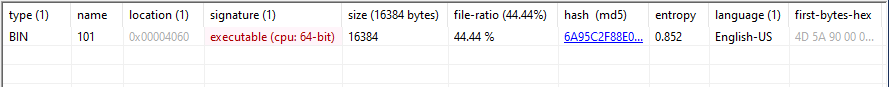
\includegraphics[width=0.85\textwidth]{pestudio-resources-exec}
\caption{Esempio di risorsa malevola contenuta in un file PE analizzata con PEStudio. In questo caso si può notare che come risorsa è stato inserito un eseguibile.}
\label{fig:pestudio-resources}
\end{figure}

Molto importante è la sezione \softwarecommand{strings} che ci mostra le stringhe trovate dall'analisi del file PE. La figura\ref{fig:pestudio-strings} mostra le come vengono rappresentate le stringhe e come PEStudio suggerisce già i possibili utilizzi delle stringhe. Analizzando con PEStudio un esempio di keylogger potremmo trovare all'interno le seguenti stringhe:

... elenco stringhe
... descrizione delle stringhe.\\

\begin{figure}[H]
\centering
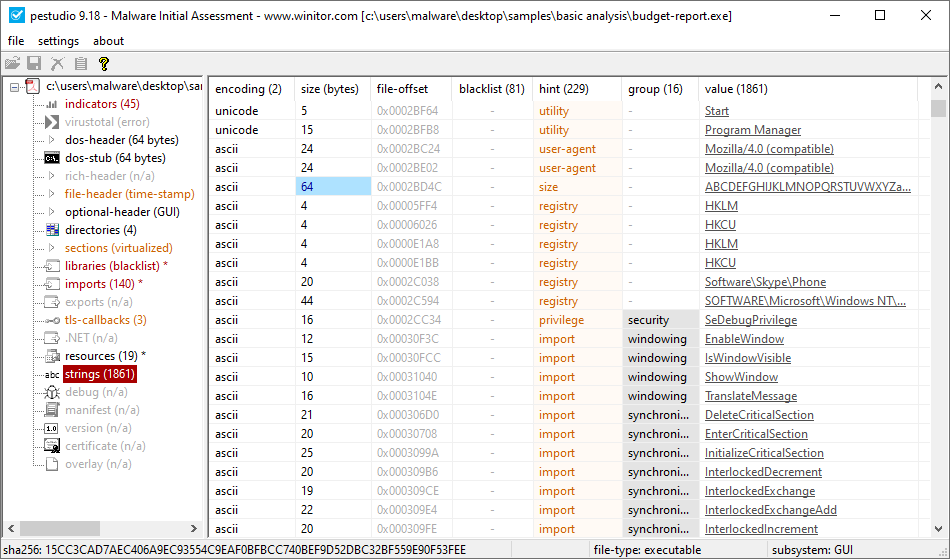
\includegraphics[width=0.65\textwidth]{pestudio-strings}
\caption{Elenco delle stringhe trovate all'interno di un file PE con l'analisi delle stringhe in PEStudio.}
\label{fig:pestudio-strings}
\end{figure}

La funzione \strings{Sleep} è spesso un segnale d'allarme poichè viene utilizzata dai malware per aggirare software antivirus o anti-malware.

Altre sezioni meno importanti per l'analisi sono \softwarecommand{directories}, che indica le data directories.

Un problema che può sorgere nell'analisi di un malware è il fatto che il malware può essere impacchettato. Per analizzare un malware impacchettato bisogna prima spacchettarlo. Per fare ciò si rimanda al capitolo sull'offuscamento.

\subsection*{\softwarename{PEView}}
Un altro software per l'analisi di un file PE è PEView. A differenza di PEStudio ...\\

Per analizzare un file con PEView la prima cosa da fare è avviare il programma con i privilegi di amministratore e verrà subito chiesto di selezionare dalle cartelle il file malevolo da visualizzare. Una volta fatto ciò PEView mostra i dati contenuti nel file PE come in figura \ref{fig:peview-main}. \\

\begin{figure}[H]
\centering
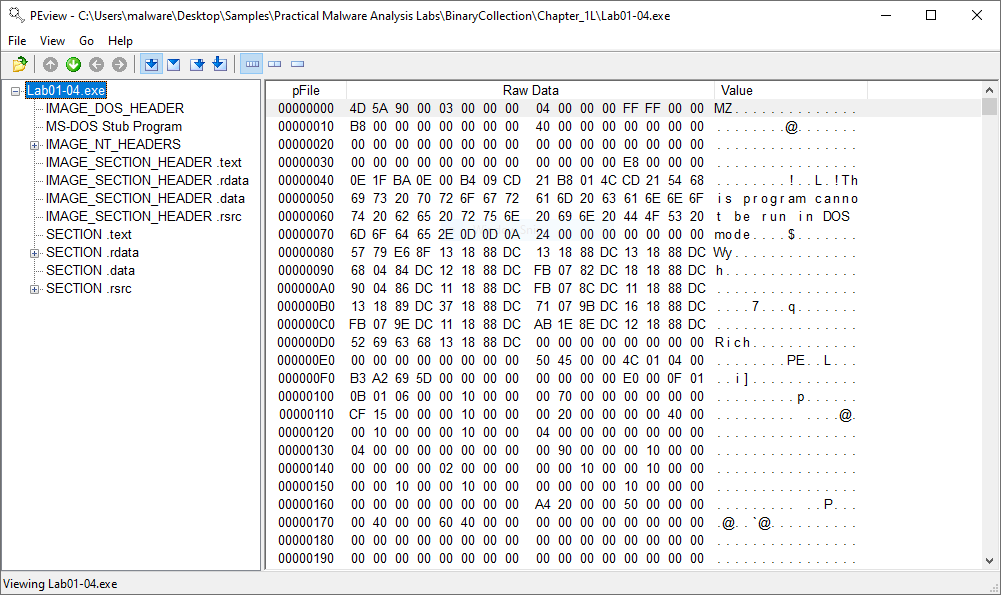
\includegraphics[width=0.65\textwidth]{peview-main}
\caption{Schermata iniziale mostrata da PEView al caricamento di un file.}
\label{fig:peview-main}
\end{figure}

Nella parte sinistra della finestra di PEView è possibile vedere anche il contenuto delle sezioni dell'eseguibile e dei vari header. Spesso all'interno dei malware viene inserito del codice eseguibile all'interno della sezione dedicata alle risorse; con PEView è possibile identificare eventuali risorse eseguibili. Nella figura \ref{fig:peview-addresstable} è possibile vedere il contenuto dell'import address table.\\

\begin{figure}[H]
\centering
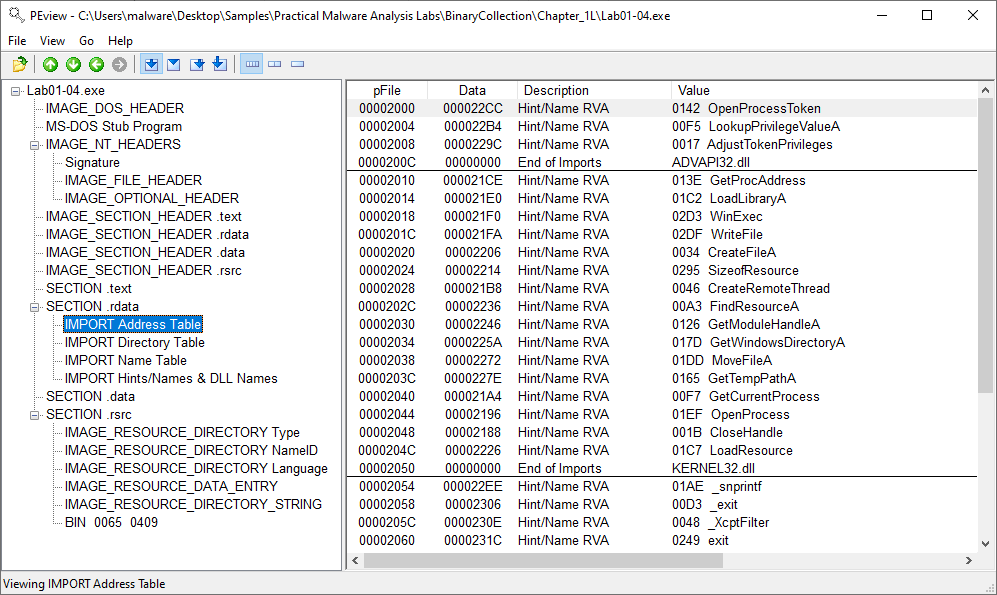
\includegraphics[width=0.65\textwidth]{peview-addresstable}
\caption{Sezione di un file PE contenente la Import Address Table visualizzata con PEView.}
\label{fig:peview-addresstable}
\end{figure}

\subsection*{\softwarename{CFF Explorer}}
Consente anche di modificare eventualmente i campi del PE file.

%%%%%%%%%%%%%%
%% analisi dinamica di base
\chapter{Analisi dinamica di base}

%%%%%%%%%%%%%%%
%% analisi statica avanzata
\chapter{Analisi statica avanzata}

\section{Reverse Engineering}

\subsection*{\softwarename{IDA Freeware}}
\subsection*{\softwarename{Ghidra}}
Questo software è stato progettato dalla NSA (National Security Agency) americana.

%%%%%%%%%%%%%%%%
%% analisi dinamica avanzata
\chapter{Analisi dinamica avanzata}

\subsection*{\softwarename{x32dbg}}

%%%%%%%%%%%%%%%
%% analisi dei pdf e javascript
\chapter{Analisi di script e documenti}

\section{Analisi di documenti PDF}
\subsection{Struttura di un PDF}
\subsection{Analisi di un PDF}

\section{Analisi di codice Javascript}

%%%%%%%%%%%%%%%%
%% tecniche di offuscamento
\chapter{Tecniche di offuscamento}

\section{Modifica delle stringhe}
Gli attaccanti possono tentare di rendere difficile l'analisi delle stringhe inserendo all'interno del programma stringhe casuali o di tutt'altro significato volte a far credere che il file non sia un file malevolo.

In alcuni casi possono cifrare delle stringhe per oscurarne il contenuto oppure usare dei sistemi di codifica in base64. L'utilizzo di una codifica in base64 all'interno del malware può essere indicata, tramite l'analisi delle stringhe, dalla presenza di stinghe come ABC...abc...+/. Si faccia riferimento al capitolo 2(?).
Può essere utilizzata anche la codifica XOR. Il problema di utilizzare una codifica XOR è il fatto che, a causa della presenza del carattere nullo alla fine di una stringa, riesco a riconoscere la chiave e recuperare l'intera stringa.

\section{Impacchettamento}

\subsection{Come spacchettare un malware}
Ci sono diverse tecniche per fare l'unpacking di un malware.

\subsubsection*{UPX}
Nel caso un malware sia impacchettato con UPX si può scaricare il software upx e dal terminale dare il comando:\\
\shellcommand{upx -d -o <percorso\_output> <percorso\_malware>}
dove \scommand{<percorso\_output>} corrisponde al percorso in cui volete salvare il file spacchettato, includendo anche il nome del nuovo file, mentre \scommand{<percorso\_malware>} corrisponde al percorso in cui si trova il malware da spacchettare. Nella figura \ref{fig:upx-output} è mostrato l'output risultante se l'operazione va a buon fine.

\begin{figure}[H]
\centering
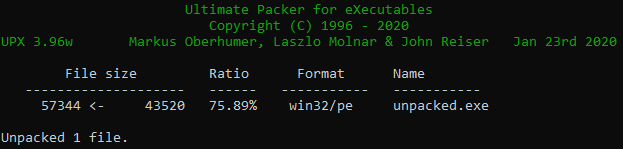
\includegraphics[width=0.7\textwidth]{upx-output}
\caption{Messaggio che viene mostrato dopo aver eseguito UPX per spacchettare un file e salvarlo in un altra cartella.}
\label{fig:upx-output}
\end{figure}

%%%%%%%%%%%%%%%%%%%%%%%%%%%%%%%%%%%%%%%%%%%%%%%%%%%
\appendix

%%%%%%%%%%%%%
%% appendice windows
\chapter {Sistema operativo Windows}

%%
\section{Librerie ed API in Windows}
Le librerie più comunemente utilizzate in Windows sono riassunte nella seguente tabella e verranno analizzate singolarmente citando le funzioni più importati.

\subsection{Kernel32.dll}
\subsection{Advapi32.dll}
\subsection{User32.dll}
\subsection{Gdi32.dll}
\subsection{Ntdll.dll}
\subsection{WSock32.dll}
\subsection{Ws2\_32.dll}
\subsection{Wininet.dll}


%%
\section{Formato Portable Executable}
Il formato PE (o Portable Executable) è un formato di file molto importante durante l'esecuzione di un file eseguibile. Il Loader, che si occupa di caricare in memoria l'eseguibile, deve caricare il codice del file, la sezione Data e importare le librerie. Per sapere tutte le informazioni per allocare lo spazio di memoria corretto e le librerie utilizzate da caricare utilizza il file PE. Il file PE contiene al suo interno informazioni come quanto spazio di memoria deve essere allocato per eseguire un file .exe, quali librerie o file DLL caricare, come sono divise le sezioni all'inteno dell'eseguibile ovvero dove finisce il codice e iniziano i dati. 

Il Loader quando alloca lo spazio di memoria da un file PE, associa un indirizzo di memoria che punta alla sezione allocata chiamato \textbf{Image Base}, inoltre il file PE ha un relative virtual address, che parte dalla prima sezione di memoria del PE e non è quindi assoluto. Per recuperare una certa allocazione nello spazio dedicato al file PE bisognerà calcolare: $ImageBase + RelativeVirtualAddress$.

Nel PE file ci possono essere anche informazioni su come viene eseguito il file .exe, ad esempio se il programma è un programma che viene lanciato da linea di comando oppure se ha un'interfaccia grafica. Un file PE è composto da diverse sezioni o header:
\begin{itemize}
\item DOS Header
\item PE Header
\end{itemize}

\subsection{DOS Header}
La prima componente di un file in formato Portable Executable è il DOS Header.  Questo è rappresentato dalla struttura sottostante che si trova all'interno dell'header winnt.h:

... struttura DOS header

e\_lfanew è un puntatore al header successivo, ovvero il PE Header.

\subsection{PE Header}
Il PE Header è una struttura di tre elementi: una signature, il File Header e l'Optional Header. La signature è una stringa ascii dal valore "PE" per indicare che il file in questione è un file PE.

\subsection{File Header}
In questo header ci sono quattro campi che servono a dare informazioni sul file corrente. Il primo campo è Machine che indica l'architettura su cui  l'eseguibile è stato progettato per girare: se a 32 bit (014C) o a 64 bit (8664). Un altro campo è il TimeDateStamp che indica quando il file è stato compilato in seconda dal 31 dicembre 1969 alle 4 PM. Il NumberOfSections indica il numero di sezioni contenute all'interno del PE file. L'ulimo campo sono le caratteristiche: una struttura con un insieme di flag e in base a quale flag è settato capiamo che tipo di file si ha davanti.

\subsection{Optional Header}
L'Optional Header è un altra struttura che, nonostante il nome, non è opzionale ed ha all'interno molti campi.

... struttura
... descrizione di tutti i campi.

\subsection{Section Header}
.text: contiene il codice da eseguire.
.data: contiene sia variabili globali o statiche il cui valore è stato inizializzato al momento della compilazione
.bss: contiene dati non inizializzati
.idata: contiene la import address table.
edata: contiene funzioni esportate dalla libreria.
.reloc: ???
.rsrc: risorse

Per ciascuna sezione esiste un header con valore Name di un byte che ci indica il nome, VirtualAddress, PointerToRawData, VirtualSize e SizeOfRawData. Esiste anche un campo Characteristics che contiene i permessi di una sezione, ovvero di scrittura, lettura ed esecuzione. 
.text deve essere sia leggibile che eseguibile
.data deve essere sia leggibile che scrivibile.

\subsection{Risorse}
Possono essere icone, immagini o qualsiasi componente dell'interfaccia grafica di un file eseguibile.

%%
\section{Registro di sistema}

%%%%%%%%%%%%%
%% appendice assembly
\chapter{Linguaggio Assembly}
In questa sezione si illustrerà in maniera sintetica il funzionamento del linguaggio Assembly x86 al fine di comprendere il processo di disassemblaggio del codice malevolo che si vuole analizzare.

\section{Registri della CPU}
I registri si dividono in categorie: registri \textbf{generali}, registri di \textbf{segmento} e \textbf{flag di stato}.

\subsection*{Registri generali}
Detti anche \textit{general-purpose registers}, sono registri che hanno lo scopo di memorizzare dati o indirizzi di memoria. Qui di seguito sono elencati i principali registri a 32 bit:
\begin{itemize}
\item \textbf{EAX}: utilizzato per memorizzare i valori di ritorno delle funzioni;
\item \textbf{EBX}: utilizzato come \textit{base pointer} alla data section;
\item \textbf{ECX}: utilizzato come contatore per le stringhe e per i cicli;
\item \textbf{EDX}: puntatore I/O;
\item \textbf{ESI}: \textit{source pointer} per operazioni con le stringhe;
\item \textbf{EDI}: \textit{destination pointer} per operazioni con le stringhe;
\item \textbf{ESP}: utilizzato come \textit{stack pointer};
\item \textbf{EBP}: Stack frame base pointer;
\item \textbf{EIP}: detto anche "Instruction pointer", memorizza l'indirizzo della prossima istruzione da eseguire.
\end{itemize}

\subsection*{Registri di segmento}
...

\subsection*{Flag di stato}
I flag di stato servono a ++

\begin{figure}[!ht]
\centering
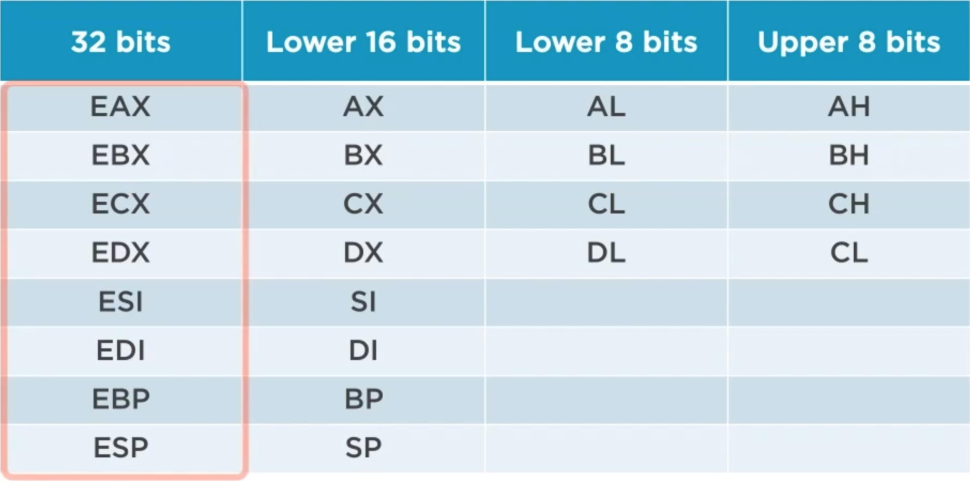
\includegraphics[width=0.8\textwidth]{general-registers}
\caption{Tabella che rappresenta i registri generali e i nomi assegnati in base ai bit presi in considerazione.}
\end{figure}

\section{Endianess}
Specifica l'ordine in cui viene memorizzato un codice esadecimale associato ad una procedure. In poche parole si decide da che parte deve stare il byte meno significativo. Si può distinguere tra \textbf{Big Endian} e \textbf{Little Endian}.\\

Se si parla di \textbf{Big Endian}, un eventuale indirizzo esadecimale 0x12345678 viene salvato così com'è scritto, ovvero con il carattere più significativo a sinistra. Big Endian si utilizza all'interno dei pacchetti di rete.

Con il \textbf{Little Endian} invece, l'indirizzo utilizzato precedentemente verrà salvato come 0x78563412 (si ricorda che raggruppiamo i caratteri su 8 bit quindi si considerano coppie di caratteri esadecimali), ovvero con il byte più significativo a destra. Questa tipologia viene utlilizzata per salvare gli indirizzi in memoria RAM.

\begin{figure}[!ht]
\centering
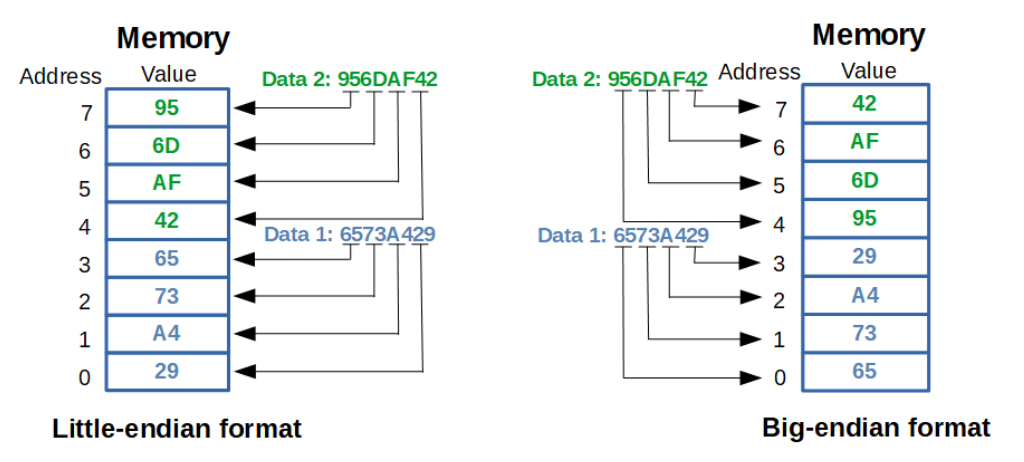
\includegraphics[width=0.8\textwidth]{endianess}
\caption{Rappresentazione del salvataggio degli indirizzi secondo le politiche di Endianess.}
\end{figure}

\section{Istruzioni}
Le istruzioni 

\end{document}

